%File: formatting-instruction.tex
\documentclass[letterpaper]{article}
\usepackage{aaai}
\usepackage{times}
\usepackage{helvet}
\usepackage{courier}
\usepackage{graphicx}
\usepackage[utf8]{inputenc}

\frenchspacing
\setlength{\pdfpagewidth}{8.5in}
\setlength{\pdfpageheight}{11in}
\pdfinfo{
/Title (Control of a Robot Arm with Artificial and Biological Neural Networks)
%/Author (Abraham M. Shultz, Sangmook Lee, Thomas B. Shea, Holly A. Yanco)}
\setcounter{secnumdepth}{0}  

\newcommand{\superscript}[1]{\ensuremath{^{\textrm{\scriptsize{#1}}}}}
\newcommand{\subscript}[1]{\ensuremath{_{\textrm{\scriptsize{#1}}}}}

\begin{document}
% The file aaai.sty is the style file for AAAI Press 
% proceedings, working notes, and technical reports.
%
\title{Control of a Robot Arm with Artificial and Biological Neural Networks}
\author{Abraham M Shultz, Sangmook Lee, Thomas B. Shea, Holly A. Yanco\\
University of Massachusetts Lowell\\
One University Avenue\\
Lowell, Massachusetts 01854\\
}
\maketitle
\begin{abstract}
\begin{quote}
To perform research on learning in cultures of mouse neurons, a hardware and software system for interfacing a biological neuronal culture to a robot arm has been constructed. 
The software architecture is modular, which permits simulated neurons to be used in place of biological neurons. 
In both cases, the activity of the culture over time is represented as an activation vector that captures recent spatiotemporal patterns of neuron firing. 
The activation vector is converted into control signals for the arm in a manner that can be generalized to multiple degrees of freedom. 
Preliminary results from the system with both simulated and biological cultures are presented. 
\end{quote}
\end{abstract}

\section{Introduction}

To study the behavior of small networks of biological neurons, the neurons can be cultured \textit{in vitro}. 
Growing the neurons as a culture allows them to be examined more easily than they could be in a living organism. 
However, living organisms have constant experience of the outside world through their senses. 
This embodiment is crucial to the development of the organism as a competent being in the world.
Embodiment allows the pre-existing structures of the brain to acquire their full development by reinforcing those connections which lead to successful action, and diminishing those which result in failure. 
Many roboticists have also noted the need for embodiment of algorithms \cite{brooks1991intelligence,chiel1997brain,anderson2003embodied}. 

We do not propose that biological neurons in culture will be able to develop into an effective controller for a robotic system.
Neurons are very sensitive to their environment, and can only live in a very narrowly proscribed range of conditions. 
Outside those conditions, or if the culture is contaminated by bacteria, the neurons die. 
Additionally, each culture is unique. Multiple cultures may be created with similar initial conditions, but the cells will be uniquely laid out and connected. 
As a result, while one can make broad and statistical assertions about their behavior, there is not a high level of inter-cultural similarity at the level of individual signaling patterns. 

The fact that biological cultures, as currently used, do not make a robust and repeatable robot controller does not mean that embodying neuronal cultures in robotic systems is useless. 
Rather, embodiment provides us with a means of learning about the connectivity and growth of neurons in culture. 
To that end, we have constructed a closed loop of perception, stimulation, activation, and action that allows cultured mouse neurons to interact with the real world using a Manus ARM robot.

\section{Methods}

There are two components of this research. 
The first component is the growth of biological neuronal networks for use as robotic controllers; the second is the simulation of these cultures \textit{in silico} to guide future research. 
To reach our goal of accurately simulating the biological networks, we are using the observed behavior of the cultured neurons to guide the development of the software for the simulator.
As the simulator's accuracy improves, it will be able to be used to simulate very large series of experiments in order to guide future research with biological cells in useful directions. 

\subsection{Biological Cultured Neuronal Networks}

In order to gather information about the behavior of neurons, neurobiology researchers grow cultures of neurons.
A Multi-Electrode Array (MEA) is a type of culture dish that provides researchers with a way to monitor the electrical activity of neurons at or near the level of individual cells. 
These cultures of neurons also allow the researchers to perform experiments that operate directly on the neurons, without the complications that may be caused by the interacting systems of a living organism. 
Research in The Center for Cellular Neurobiology and Neurodegeneration has used this method with bicuculline to demonstrate that inhibitory connections are required for learning in cultured neurons, and with amyloid-$\beta$ to demonstrate its effects on signaling \cite{lee2013rapid,shea2009optimization}. 

Despite the advantages of cultures, they also have drawbacks. 
Complete organisms receive stimulation from their senses for their entire lives. 
Before birth, the genetic and chemical signaling within the organism organizes and differentiates the developing neuronal tissue into specialized layers and structures. 
For some time before birth, and continuously after the organism is born, incoming sensory information is handled by the pre-existing organization within the brain to form impressions of the outside world. 
In culture, a neuronal network does not receive stimulation unless it is provided by the researcher. 
Such stimulation accelerates the development of the culture towards its mature state, indicating that the neurons still develop in a way similar to the way they would in a complete brain \cite{zemianek2012accelerated}.

The propagation of impressions through the brain results, eventually, in motor activity, which in turn changes the organism's relation to the world and the resulting sensory input. 
This complete loop is what we mean when we talk about \textit{embodiment}: the ability of a system to perceive the outside world, process that perception, and act in the world. 
The brain closes the gap between perception and action, while the world closes the loop between action and perception. 
By embodying neuronal cultures in a robot, our goal is to provide a system for investigating how incoming signals are integrated by neuronal networks, and how this integration affects the structure of the network. 

\subsection{Construction}
The MEA itself consists of a glass plate with an array of conductive pads laid out on it. 
Conductive traces extend from each pad to the edges of the plate. 
When a neuron sends a signal, its electrical potential changes, and this change in potential is detected by sensitive amplifiers connected to the traces for pads near that neuron.

Fetal mice are used as the cell source because their neurons are still developing and forming connections. 
To acquire cells, mice must be bred and sacrificed, and the fetal mouse neural tissue must be surgically prepared and chemically treated before being plated on the MEA. 
The chemical treatment uses enzymes to disassociate the individual neurons. 
The neurons are added to the MEA as a suspension in liquid medium and given some time to bond to the MEA.
After the neurons have bonded, the culture medium is replaced, which removes any unbonded cells along with the old culture medium \cite{wagenaar2006extremely}.
Typical cell suspension densities range from 300 to 2,000 cells per mm$^2$, but can reach as high as 80,000 cells per mm$^2$ \cite{shea2009optimization,ruaro2005toward}.
Extremely sparse cultures tend to have high mortality rates and do not form sufficient connections to display mature signaling patterns \cite{shea2009optimization}.

Since the culture is applied to the plate as a suspension of neurons, there are limited ways to control the location and distribution of neurons. 
One method is to apply the suspension of neurons to the desired regions using a micropipette, resulting in higher neuron density in areas where the drops were added. 
Another method is to apply pattern of protein that affects how the neurons bond to the plate surface.
The pattern of cells influences the connectivity of the culture \cite{sorkin2006compact}.

When the cells are initially added to the culture, they are not connected, but they begin to form connections quickly.
Starting at around 7 days \emph{in vitro} (DIV) and continuing to around 30 DIV, the connections are not complete, and signaling is dominated by constant, high-amplitude spiking \cite{warwick2010controlling}. 
The resulting signals have been described as ``epileptiform."
In the young, epileptiform stage, it is impossible to isolate the neurons' response to stimulus from the constant spike activity, so experiments must be performed after the neuron network is finished developing. 

After the initial period of epileptiform activity, the cells enter a ``mature" phase, characterized by sparse bursts of spikes separated by quiet periods. 
The active bursts may be localized to one region, spread across the culture, or propagate from region to region. 
After 2-3 months of this type of activity, the culture eventually becomes senescent, and only reacts to stimuli in simple, stereotyped ways \cite{warwick2010controlling}. 
The cells can continue to live for months or even years, assuming that equipment failure or bacterial infection does not kill them \cite{potter2001new}. 

\subsection{Robot}

The robot used in this work is a Manus ARM (Assistive Robotic Manipulator), created by Exact Dynamics.
The ARM is a 6-DOF arm with a two-fingered gripper. 
A Microsoft LifeCam 720p resolution webcam is mounted on the gripper (Figure \ref{fig:cam_on_gripper}) to serve as a source of feedback to the cultured neurons. 

%\begin{figure}
%	\centering
%	\includegraphics[width=\columnwidth]{full_arm.png}
%	\caption{The arm with mounted camera. The camera is the black cylinder with a silver end on top of the gripper.}
%	\label{fig:full_arm}
%\end{figure}

\begin{figure}
	\centering
	\includegraphics[width=\columnwidth]{gripper_cam.png}
	\caption{The gripper with mounted camera.}
	\label{fig:cam_on_gripper}
\end{figure}


When the ARM moves, the camera moves with it, changing the view of the world. 
The image from the camera is converted to HSV color space and thresholded to find concentrations of red pixels.
The stimulation signal is a recording of neuronal activity from cultured neurons, as described in Zemianek et. al. \shortcite{zemianek2012stimulation}.
This stimulation provides feedback to the culture about the state of the world, and the culture's reaction to the stimulus provides motion commands to the arm to move in the world. 

\begin{figure*}
	\centering
	\includegraphics[width=\textwidth]{full_system_horizontal.eps}
	\caption{Diagram of the full system. Hardware on the left side of the diagram is located in the Robotics Laboratory, hardware to the right side is located in the Center for Cellular Neurobiology and Neurodegeneration.}
	\label{fig:full_loop}
\end{figure*}
% Server image is from http://www.public-domain-photos.com/free-cliparts/computer/other/server_mimooh_01-2531.htm and they say it's free/libre. 


At present, the red pixel concentrations on the left and right sides of the image are used to determine whether the culture should be stimulated on the corresponding side. 
The current motion control scheme is one-dimensional because the currently available stimulation hardware provides only two input channels, and this creates a bottleneck for feedback to the biological culture. 
By developing a more complex stimulation system, particularly one which can apply a pattern of activity over some or all of the available stimulation sites, the complexity of the input to the culture can be increased. 
More complex stimulation will provide a more versatile representation of the view from the camera, expanding the dimensionality of the input stimulus and thus the expected dimensionality of the output.

\subsection{Computer Interface}

In order to read neuronal signals from the culture, the MEA is placed in a MEA1060-INV amplifier manufactured by Multi Channel Systems GmbH. 
The amplifer has 60 channels, one for each contact pad of the MEA.
Each channel has a fixed gain of 1200.
The amplifier outputs are connected to a PCI-6071E DAQ card manufactured by National Instruments. 
The card is controlled through the Linux COntrol and MEasurement Device Interface (COMEDI), which provides an open source library for collecting data from DAQ cards. 

The acquisition and processing software is maintained as a collection of ROS (Robot Operating System) nodes \cite{ROSAnnouncementPaper}.
The node which acquires data from the DAQ card is called ``Zanni.''
Zanni samples the card 1000 times per second and outputs the current value in volts of each channel of the MEA. 
A collection of 60 voltage values is referred to as a ``dish state'' because it represents the electrical activity of the MEA at a specific instant in time. 

Dish states are collected by a ROS node which uses the time series of voltages in each channel to determine the mean and standard deviation of the electrical signal. 
In order to determine the mean and standard deviation, the node first buffers 3000 dish states from which to calculate the mean and standard deviation, the number of dish states buffered can be set from a configuration file. 
Any time that the signal on a channel increases beyond 3 standard deviations from the mean for that channel, the channel is considered to be ``spiking.'' 
A spike on a channel indicates that a neuron near the conductive pad for that channel has produced an action potential. 
However, the mapping of neurons to pads is not 1-to-1, so activity on a channel may indicate a small group of nearby neurons, rather than a single specific neuron.

In order to convert spikes from the culture into motion commands for the arm, a simplified version of the control scheme from DeMarse \textit{et al}. \shortcite{demarse2001neurally} is used. 
For each channel in the dish, if a spike is detected on that channel, the activation A at that site is incremented and decayed by: 

$A_n (t_i) = A_n(t_{i-1})e^{-\beta(t_i - t_{i-1})} + 1$

\noindent Activation decays exponentially over time with the decay constant $\beta=1s^{-1}$.
The activations over the entire culture are collected in the activation vector V, and normalized to the range 0.0 - 1.0 by applying

$V_n(t_i) = tanh(\delta A_n(t_i))$

\noindent with $\delta=0.1$. Without normalization, recording sites with very high spike rates can dominate the output, even if the variation of the site in response to stimulation is minimal. 
The resulting vector of 60 floating-point values is the normalized activation vector for the dish at a specific time.
Every 0.2 seconds, the normalized activation vector of the culture is compared to a pair of pre-selected activation vectors. 
The pre-selected vectors are a ``right'' and ``left'' vector, with the ``left'' vector having maximum activation at all pads on the left side of the dish and zero elsewhere, while the ``right'' vector has maximum activation at all pads on the right side of the dish and zero elsewhere. 

The comparison is a simple calculation of Euclidean distance between the left and right vectors and the current activity vector of the culture. 
If the distance from the current activation vector to the left vector is less than the distance to the right vector, the arm will be commanded to move left. 
Similarly, if the current vector is closer to the right than the left vector, the arm will be commanded to move right. 
In either case, the difference between the distances must be large enough to overcome a dead band, or the arm is not instructed to move at all. 
Because it uses two constant vectors for comparison, this system only permits motion left or right, along a single axis. 
By expanding the selection of vectors used for the comparison, additional degrees of freedom could be controlled. 

\subsection{Simulated Cultured Neuronal Networks}

Because each biological culture is labor-intensive to grow but easy to kill, simulating cultures could be a useful approach to early phases of experimentation. 
In order to simulate a full MEA, the simulator must model the dispersal of cells over the surface of the MEA, the networking of those cells, and their activity. 
The first part of the simulator decides the distribution of the cells over an area according to the density of the desired culture and the surface area of the MEA plate. 
The process of determining the cell locations is called ``plating."
After the plating simulation has placed the cells, a growth simulation uses the locations of the cells to determine how the individual neurons are connected to form the network. 
In order to decide which neurons are connected, mathematical models based on the observed networking behavior of real neurons are used \cite{abe2013control}. 
The output of the plating and growth simulations is the connectivity map of a biologically plausible neuronal network.
There does not currently exist any method to determine the complete connectivity of a biological neuronal network, but as imaging and analysis techniques improve, the information they reveal can be incorporated into the simulation. 
Eventually, the simulation system may be able to model a specific culture at a sufficient level of detail to predict the biological network's activity.

\subsection{Plating simulation}

In a typical MEA, the cells are plated on glass prepared with binding proteins, allowed to bond, and then washed, so any cells that are not in contact with the glass are removed.
As a result, all of the cells in the culture are in a single layer on the glass of the MEA.
For the purposes of the plating simulation, the layout of the simulated cells is simplified into a planar grid. 
Each square of the simulated grid is approximately the size of a single neuron cell body (30$\mu$m), and the full grid is 2500$\mu$m square.
These parameters are configurable in the simulation software to support different types of cells or configurations of MEA.

Cells are distributed on the grid according to a midpoint displacement fractal algorithm, also known as a plasma fractal \cite{Fournier1982Stochastic}. 
For our simulator, a midpoint displacement fractal was chosen to set the distribution of cell adhesion probabilities because of the similarity of its results to turbulent flows. 
The uneven distribution of cells in dishes is supported by the uneven areal density of cultures, as seen in Shea \citeyear{shea2009optimization}. 

As an alternative to the plasma fractal, the simulator also allows the use of an image to specify the cell occupancy probabilities. 
The red channel of the image is mapped to the grid of points on the dish, with the saturation of color at each point used as the probability of that point containing a cell. 

After the probability of cell placement at each location in the dish is determined, the plating simulation marks each location as occupied or not, based on the probabilities of a location having a cell and the density of cells in the plating solution. 
Those locations that are marked as occupied are treated as having a cell on them. The others are assumed to be empty space. 

After the cell locations are determined, there are a series of pruning steps that are intended to simulate cell deaths in the culture. 
In biological cultures, 45-60\% of the cells die before the network is done wiring itself, within approximately the first 17 DIV \cite{erickson2008caged}.
Because so many of the cells die off, they do not need to be considered when the simulation begins to determine network connectivity. 
In order to model the early cell mortality, the locations that the simulator has marked as occupied are decimated based on the observed survival probabilities of cells in culture. 

%\subsection{Connectivity and Growth}

Typical cell suspension densities are in the range of 300-2000 cells/mm\superscript{2}, resulting in 1200-8000 cells in the active area of the MEA and so millions of possible connections if each cell could connect to any other cell \cite{wagenaar2006extremely}.
However, there are limits on cell growth and networking which make the computation of the network connectivity more tractable. 
Chemical interactions between cells restrict the number of connections that should be considered when developing the connectivity of the dish. 

Kahng, Nam, and Lee \shortcite{kahng2007stochastic} provides a model based on observation of chemotaxis in developing neurons, but simplified into a stochastic model. 
The growing end of an axon moves in a random walk on a grid. 
Each step may take it in any of 8 directions: up, down, left, right, or the four diagonals.
If, after making a step, the walking point is with 20$\mu$m of a dendrite of another neuron, the two neurons are considered connected. 
The probability of a connection between two cells is effectively a function of the distance between them, which makes it unlikely a cell will connect to itself, but likely it will connect to neighbors, and unlikely that it will reach very far \cite{Segev2000185}. 

Our simulator uses a Gaussian distribution to model the probability of a pair of cells connecting based on the straight-line distance between them, with parameters set to maximize connectivity around 200$\mu$m from the cell body. 
The Gaussian distribution also provides a limitation on the number of possible connections that must be considered by the program during the growth simulation. 
If the distance between two cells is so large that the probability of a connection between them is vanishingly small, it may be disregarded when the network is being laid out, thus saving computation time. 

In addition to the limits imposed by chemotaxis, observations of the connections in MEAs indicate that only 20-50\% of the possible connections are made. 
Patel, Scott, and Meaney \shortcite{patel2012dynamic} indicate that the out-degree of cortical neurons can be modeled using a Poisson distribution with a mean of 22. 
Allowing such a stochastic distribution of connectivity will cause some neurons to be extremely well connected while others are less connected. 
Such patterns of connectivity are seen in biological cultures, so the Poisson distribution is used in the simulation to set the out-degree of the neurons. 
Once a neuron forms a number of connections equal to its selected out-degree, no further connections from that neuron are considered, although other neurons may still connect to it.

Once the model is completed, it may be run, and voltage and spike train data collected from it. 
Since each neuron is in a known location in the simulated culture, the simulation selects the neurons located on or near the conductive pads for a given MEA layout, and records data from those neurons. 

\subsection{Neuron models}

For initial development, the cell model used was a simple leaky integrate-and-fire (LIF) model. 
The LIF model was chosen because it can approximate the spike timing of a living neural network to a high degree of accuracy \cite{kahng2007stochastic,jolivet2004generalized}. 

However, while a LIF model can match the spike timing of a living network, it does not produce biologically plausible action potentials. 
That is, the events that the simulator regards as spikes are timed like those of a biological network, but the simulated membrane voltages of the simulated neurons are unlike those of biological cells. 
To obtain more realistic spike and sub-threshold voltages, the simulator was converted to use Izhikevich's integrate and fire model instead of basic LIF neurons \cite{izhikevich2003simple}.
Izhikevich's model has parameters that can be configured to reproduce the behavior of many biological neurons. 
Our simulator uses the configuration that Izhikevich calls ``Regular Spiking'' for excitatory neurons and ``Fast Spiking'' for inhibitory neurons, based on the observed behavior of biological neurons \cite{Izhikevich01082004}.

\section{Example}

\subsection{Control with a Biological Culture} 

To assess the ability of the arm to respond to signals from the culture, the arm camera was shown a tracking target on the left or right side of the camera's field of view.
The position of the tracking target affects the stimulation of the culture, and the reaction of the culture to the stimulation would trigger motion in the arm. 
The resulting motion of the arm was recorded by rosbag, a utility which records all of the activity of the ROS nodes. 
Each motion to the left was assigned a value of -1 and each motion right a value of 1. 
Starting from a center position of 0, the total motion was calculated at every timestamp where the arm was sent a motion command. 
If the arm moved left, the total motion would become increasingly negative, while right motions would cause the total motion to become more positive. 

%Picture of the motion track
\begin{figure*}
	\centering
	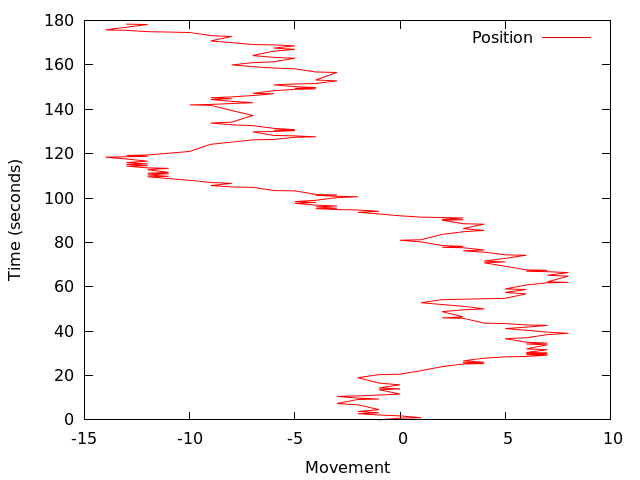
\includegraphics[width=0.3\textwidth]{bio_motion_446.png}
	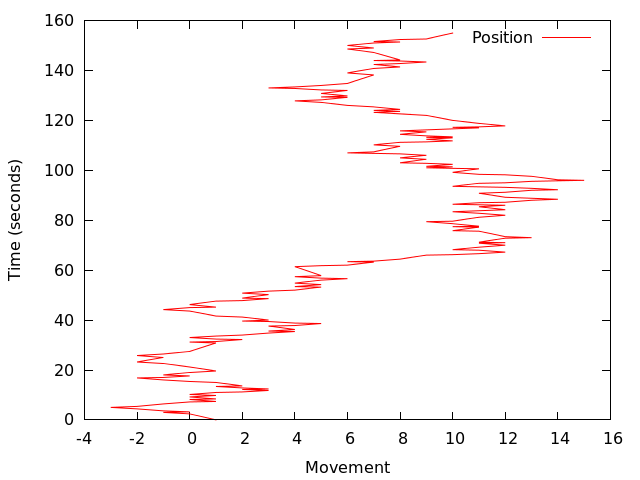
\includegraphics[width=0.3\textwidth]{bio_motion_445.png}
	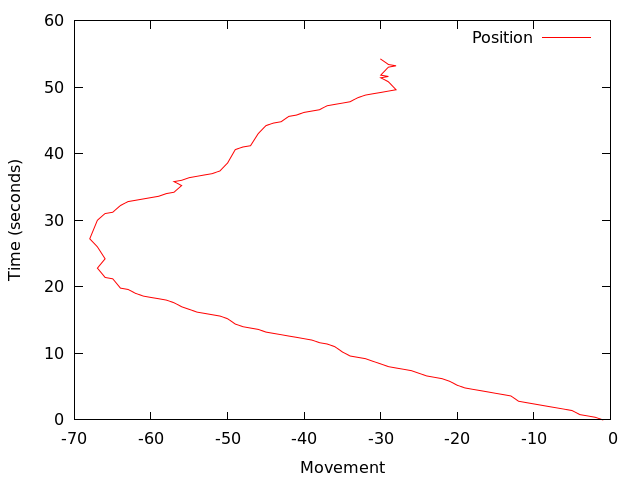
\includegraphics[width=0.3\textwidth]{simulated_motion.png}
	\caption{Movement of the arm under the control of biological and simulated neurons. In the left and center images, the system used the biological neurons as the controller. For the first image, a tracking target was presented on the left side of the field of view of the camera and the arm moved left. For the second image, the target was presented on the right, and the arm moved right. For the right image, the arm was controlled by a simulated culture which was stimulated on the left and then on the right, resulting in a movement to the left and then to the right. 0 on the movement axis is the center of the arm's range of movement.}
	\label{fig:motion_images}
\end{figure*}

Figure \ref{fig:motion_images} shows the total motion over time as the arm moved to track a target on the right side of its field of vision. 
The biological culture displays significantly more ``wiggle'' in the resulting motion than the simulated culture.
Most of this wiggle is likely due to spontaneous signaling within the culture.
However, we have some concern that some of the wiggle is an artifact of noise from outside the recording system. 
The current system displays some degree of noise at exactly 60Hz, due to interference from AC lines in the laboratory being picked up and amplified by the MEA amplifier. 
In order to suppress this noise, a software filter is being developed which will suppress 60Hz noise on each channel of the signal before attempting to classify the signal into spikes. 
%%
The expected consequence of noise in this system is to cause the reaction of the system to stimulation to have a significant degree of wiggle in it. 
Rather than cleanly responding to a left or right stimulation with left or right motion, a noisy system would have a chance that the noise would overwhelm the activity of the neurons for that time period, and result in a motion contrary to that expected from the stimulation. 
Since the stimulation would be consistent, while the noise would be effectively random, the overall motion would be correct, but interspersed with incorrect moves. 
This is what we observed in the behavior of the system under biological control.
The degree of incorrect moves is also substantially reduced in the simulated system.
The simulation does not include simulation of noise, so there is no way for noise to add incorrect moves to the motion of the arm. 

\subsection{Control with an Artificial Culture}

At present, the artificial culture cannot be run in real time. 
The computational complexity of the neuronal model and the number of neurons being simulated result in a very high load on the processor. 
In addition to this load, the python interpreter used to execute the simulation does not support parallelization across multiple processors. 
Because a less complex neuronal model would not support realistic cell membrane voltages, and reducing the number of neurons would make the simulation unlike a biological culture, using the simulator to control the arm is done in two steps. 
In the first step, the simulator is run with simulated stimulus. 
The stimulus is the same as the stimulus used in biological cultures, a pre-recorded biological signal \cite{zemianek2012stimulation}. 
Prior to the simulation run, the times that the stimulus will be delivered are configured by the software. 
Because the stimulation was recorded at 1000Hz, there is a 1:1 correlation between samples of the stimulation and timesteps in the simulation. 
The stimulation is a recording from a MEA system like the simulator is intended to simulate, and contains a voltage signal of the same amplitude as is received at the electrodes, so it is assumed that the sensing range of each pad is also the maximum reach of the stimulation applied to that pad. 
During the run, at each timestep of the simulation, the simulator determines which electrodes the stimulation should be delivered to, and what voltage should be delivered.
For each pad, the corresponding voltage is added to the membrane voltage of the neurons around the pad, in proportion to the distance between the neuron and the pad. 
After the simulation is run, the recording of all of the membrane voltages of the neurons are used to calculate the voltage at each pad. 
Each neuron contributes voltage proportional to its distance from the pad. 
The resulting voltages are recorded in a Labview LVM text file format, which many of the utilities related to the simulator are capable of processing. 

In order to control the arm using a recording, a program was written that uses the Labview LVM file as input, and publishes dish states as if the input were received from a biological culture.
Because of the modular nature of the ROS software, this program can interface to the software that generates the activation vectors and arm motion control outputs without modification of any other component of the software. 
The arm can then be run as if it were being controlled by a neuronal culture. 

When the arm is run with a simulated recording, there is no noise at all present. 
The arm moves with a very high degree of correspondence to the applied stimulation. 
For the simulated test run, the simulated culture started with 5 seconds of no stimulation, then received 20 seconds of stimulation on the left side, 10 seconds of no stimulation, 20 seconds of stimulation on the right side, and then 5 more seconds of no stimulation. 
As shown in Figure \ref{fig:motion_images}, the arm moves left, stops, and then moves right. 
The rightward motion does not completely return to the center position of the arm. 
It also displays a greater slope in the graphic, as the arm took a longer time to do less motion.
The slower motion to the right is likely because the stimulation on the left side of the dish would initiate activity that would compete with the stimulation on the right side of the dish.
Because the activity from the left side stimulation would not have died out completely by the time the right side stimulation started, the rightward motion would be interfered with. 

\section{Discussion and Future Work}

There are computational methods for determining the approximate wiring of a developed culture, based on the propagation delay of a signal in the culture and the synchrony of activity between different sites in the culture  \cite{erickson2008caged,esposti2008estimation}. 
These methods offer some promise for mapping the connectivity of the dish, but they do not give a complete or fully-accurate map. 
Even if it was possible to completely map the connections of a culture, there is no way to duplicate it, as there is no way to control the growth of individual biological neurons and their axons. 
A simulated network that uses the connectivity of an existing dish and displays the same activity patterns could be argued to be a duplicate of the culture at that time. 
Such a simulated culture could then be backed up, shared with collaborators, and preserved in ways that a biological culture cannot be. 

It will be possible to accelerate our simulator by parallelizing it on a multiprocessor computer or GPU.
The current system is written in Python, using the BRIAN simulator framework \cite{goodman2008brian}. 
Python does not support parallelization well due to design elements of the Python interpreter, but frameworks and software for simulating networks of neurons on GPUs already exist. 
As a result, our plating simulation can be used to set up the connectivity and neuron locations of the culture, but the actual execution of the network can be handed off to hardware that supports parallel operations better. 

It would be overstating the semantic content of these patterns to claim that the activity within the network represents the object that elicited the stimulus, but such pattern recognition does pave the way for two-way communication with the culture.
It may be that inhibiting signaling in response to undesired patterns of activity and exciting signaling in response to desired patterns will allow us to interactively train a culture to display certain patterns of activity. 
As described in Zemianek \textit{et al}., inversion of the stimulation signal changes whether the response at a specific site in the dish is inhibitory or excitatory \shortcite{zemianek2012stimulation}.
With a fast computer in the loop, we will be able to examine the activity of biological cultures in real time. 
This will allow us to recognize the patterns of activity that a particular input elicits in the network. 

The eventual goal for working with recognition of the patterns of activity of a neuronal network, rather than the network-wide strength of connections (e.g. DeMarse and Dockendorf \shortcite{demarse2005adaptive}), is to allow input and output streams of very high dimensionality.
Human introspective experience indicates that our sensorium is rich and detailed.
Encoding information purely as frequency of stimulation or purely as location of stimulation results in a very narrow range of representable input, and so restricts the degree of embodiment that a neuron/robot system can support.

\section{Acknowledgements}

This work was sponsored in part by Army Research Office grant W911NF-11-1-0125.

\bibliographystyle{aaai}
\bibliography{workshop-paper}
\end{document}
